\documentclass[14pt, a4paper]{article}
\usepackage{fullpage}
\usepackage[top=2cm, bottom=2cm, left=2.5cm, right=2cm]{geometry}
\usepackage{amsmath,amsthm,amsfonts,amssymb,amscd}
\usepackage{fancyhdr}
\usepackage{fixltx2e}
\usepackage{mathrsfs}
\usepackage{listings}
\usepackage{color}
\usepackage{relsize}
\usepackage{graphicx}
\usepackage[utf8]{inputenc}
\usepackage[T1]{fontenc}
\usepackage[english, russian]{babel}

\definecolor{dkgreen}{rgb}{0,0.6,0}
\definecolor{gray}{rgb}{0.5,0.5,0.5}
\definecolor{mauve}{rgb}{0.58,0,0.82}

\DeclareMathSizes{14}{24}{18}{12}

\lstset{frame=tb,
  language=Python,
  aboveskip=3mm,
  belowskip=3mm,
  showstringspaces=false,
  columns=flexible,
  basicstyle={\small\ttfamily},
  numbers=none,
  numberstyle=\tiny\color{gray},
  keywordstyle=\color{blue},
  commentstyle=\color{dkgreen},
  stringstyle=\color{mauve},
  breaklines=true,
  breakatwhitespace=true,
  tabsize=3
}

\renewcommand{\thesection}{\arabic{section}.}
\renewcommand{\thesubsection}{\thesection\arabic{subsection}.}
\renewcommand{\thesubsubsection}{\thesubsection\arabic{subsubsection}.}

\begin{document}
\pagenumbering{gobble}
\begin{titlepage}
\begin{center}
\large{БЕЛОРУССКИЙ ГОСУДАРСТВЕННЫЙ УНИВЕРСИТЕТ 

ФАКУЛЬТЕТ ПРИКЛАДНОЙ МАТЕМАТИКИ И ИНФОРМАТИКИ

КАФЕДРА ВЫЧИСЛИТЕЛЬНОЙ МАТЕМАТИКИ}
\end{center}
\vspace*{\fill}
\begin{center}
Лабораторная работа 9

\large{\textbf{Применение многочлена Ньютона для интерполирования функции}}

Вариант 7
\end{center}
\begin{flushright}
\textbf{Выполнил:}

Журик Никита Сергеевич \\ 2 курс, 6 группа

\textbf{Преподаватель:}

Будник Анатолий Михайлович
\end{flushright}
\vspace*{\fill}
\begin{center}
Минск, 2019
\end{center}
\end{titlepage}

\tableofcontents
\newpage

\newpage
\pagenumbering{arabic}

  \section{Постановка задачи}
    \begin{enumerate}
      \item
      При помощи построения многочлена Ньютона выполнить интерполирование данной функции $f(x)$;
      \item
      Вычислить теоретическую оценку и действительную невязку интерполирования;
      \item
      Проанализировать результаты и сравнить с методом наименьших квадратов и многочленом Лагранжа.
    \end{enumerate}
  \section{Алгоритм решения}
  \begin{itemize}
     \item
     Рассмотрим интерполирование исходной функции $f(x) = 1.7e^{-x} - 0.7lnx$ алгебраическим многочленом степени не выше $n$: $P_n(x) = \sum\limits_{i = 0}^n c_ix^i$ на сетке узлов $x_i = 1 + ih, i = \overline{1, 10}, h = \frac{1}{10}$.
     \item
     Для построения многочлена введём аппарат разделённых разностей. Разделённая разность $k$-го порядка определяется следующим образом: $$f(x_i, \dots, x_{i+k}) = \frac{f(x_{i+1}, \dots, x_{i+k}) - f(x_i, \dots, x_{i+k-1})}{x_{i+k}-x_i}$$
     Тогда воспользуемся формулой Ньютона для интерполяционного многочлена: \begin{equation}P_n(x) = f(x_0) + (x - x_0)f(x_0, x_1) + \dots + (x-x_0)\dots(x-x_{n-1})f(x_o, \dots, x_n)\end{equation}
     \item
     Для априорной оценки точности интерполирования воспользуемся формулой остатка интерполирования в форме Ньютона:
     \begin{equation}r_n(x) = f(x, x_0, \dots, x_n)\omega_{n+1}(x)\end{equation}
  \end{itemize}
  \section{Листинг программы}
  Для реализации алгоритма был использован Python и библиотеки numpy и matplotlib.

\begin{lstlisting}
#Newton.py

import numpy as np
from math import exp, log, factorial
import matplotlib.pyplot as plt

a = 1.0
b = 2.0
N = 10
delta = (b - a) / N
alpha = 1.7

points = [a + i * delta for i in range(N + 1)]

def f(x):
    return alpha * exp(-x) + (1 - alpha) * log(x)

def omega(k, x):
    global points
    result = 1
    for i in range(N + 1):
        if i != k:
            result *= (x - points[i])
    return result

def buildDiffs(points, f):
    A = np.zeros((N + 1, N + 2), dtype=np.double)
    for i in range(N + 1):
        A[i][0] = points[i]
        A[i][1] = f(points[i])
    for j in range(2, N + 2):
        for i in range(j - 1, N + 1):
            A[i][j] = (A[i][j - 1] - A[i - 1][j - 1]) / (A[i][0] - A[i - j + 1][0])
    return A

def prod(i, points):
    return lambda x: np.prod(np.array([(x - points[j]) for j in range(i)], dtype=np.double))

def getSolution(diffs, points):
    return lambda x: np.sum(np.array([diffs[i][i + 1] * prod(i, points)(x) for i in range(N + 1)], dtype=np.double))

def xDiff(x, diffs, points, n):
    if n == 0:
        return (f(points[0]) - f(x)) / (points[0] - x)
    return (diffs[n][n + 1] - xDiff(x, diffs, points, n - 1)) / (points[n] - x)

def deficiency(x, diffs):
    return omega(N + 1, x) * xDiff(x, diffs, points, N)

def plotDifference(samples, solution):
    space = np.linspace(a, b, samples)
    plt.plot(space, np.zeros(np.shape(space)))
    plt.plot(space, np.array([solution(x) - f(x) for x in space], dtype=np.double))
    plt.savefig("NewtonDiff.png")
    plt.show()

if __name__ == "__main__":
    A = buildDiffs(points, f)
    solution = getSolution(A, points)
    
    check = [points[0] + delta / 2.6, 
             points[5] + delta / 2.6,
             points[9] + delta / 2.6]
    
    [print("Pn({0}) = {1}".format(x, solution(x))) for x in check]
    print()
    [print("rn({0}) = {1}".format(x, solution(x) - f(x))) for x in check]
    print()
    
    space = np.linspace(a, b, 1000)
    print("Real deficiency on whole interval: " + 
          str(np.max(np.abs(np.array([(solution(x) - f(x)) for x in space], dtype=np.double)))))
    print()
    
    
    print("Expected deficiency in control points: " + 
          str(np.max(np.abs(np.array([(deficiency(x, A)) for x in check], dtype=np.double)))))
    print()
    print("Real deficiency on control points: " + 
          str(np.max(np.abs(np.array([(solution(x) - f(x)) for x in check], dtype=np.double)))))
    
    plotDifference(1000, solution)
\end{lstlisting}

  \section{Вывод программы}
\begin{verbatim}
Pn(1.0384615384615385) = 0.5753798661146216
Pn(1.5384615384615385) = 0.06346095167693704
Pn(1.9384615384615385) = -0.21865340262681887

rn(1.0384615384615385) = 4.978195078386705e-09
rn(1.5384615384615385) = -3.9230299564430027e-11
rn(1.9384615384615385) = -1.666099730401882e-09

Real deficiency on whole interval: 5.350829557215775e-09

Expected deficiency in control points: 4.978195167117301e-09

Real deficiency on control points: 4.978195078386705e-09

\end{verbatim}
\begin{figure}[h!]
  \center
  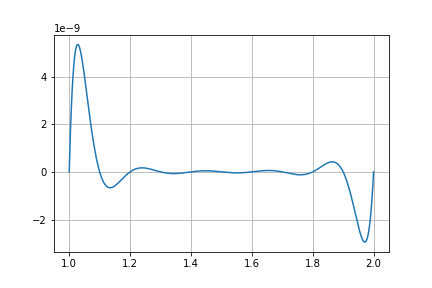
\includegraphics[width=0.6\linewidth]{NewtonDiff.png}
  \caption{Невязка интерполирования}
\end{figure}

  \section{Выводы}
  \begin{itemize}
  \item
  При интерполировании при помощи многочлена Лагранжа был многочлен, интерполирующий исходную функцию на всём промежутке с точностью $r_{Lagr_{real}} = 5.350829113126565e-09$, а в контрольных точках - $r_{Lagr_{control}} = 4.9781948563421e-09$. При использовании многочлена Ньютона были получены следующие результаты: $r_{Newton_{real}} = 5.350829557215775e-09, \ r_{Newton_{control}} = 4.978195078386705e-09$. Нетрудно видеть, что данные значения практически совпадают, что следует из того, что эти методы являются различными способами построения одного и того же многочлена.
  \item
  Сравним многочлен Ньютона с МНК. В МНК невязка в контрольных точках составила $r_{LSQ_{control}} = 9.374749135870886e-06$, что значительно больше полученной как при использовании многочлена Лагранжа, так и при использовании многочлена Ньютона. Это связано с тем, что матрица Гильберта плохо обусловлена. Таким образом, посредством многочлена Лагранжа можно добиться большей точности, чем при приближении функции методом наименьших квадратов.
  \item
  Глядя на график невязки, можно заметить, что он совпадает с графиком невязки при применении многочлена Лагранжа.
  \end{itemize}

\end{document}